\section{Comparision}\label{sec:Comparision}


\begin{figure} \centering
  {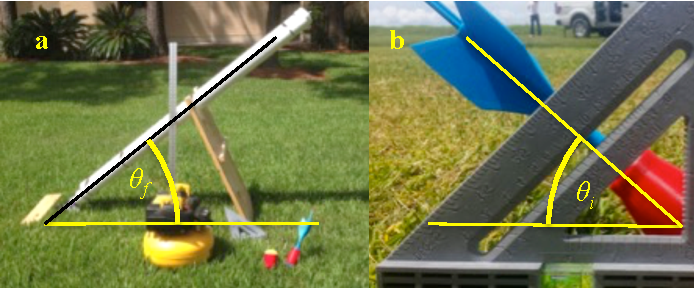
\includegraphics[width=\columnwidth]{CannonPicture}}
 \caption{A pneumatic launcher for SeismicDarts.  Ballistic dart deployment has limited usefulness because the incident angle is equal to the firing angle.} 
 \label{fig:CannonPicture}
\end{figure}

\begin{figure*}[htb]
\centering
\renewcommand{\figwid}{0.5\columnwidth}
\begin{overpic}[width =\figwid]{sim1_1.pdf}
\end{overpic}
\begin{overpic}[width =\figwid]{sim1_2.pdf}
\end{overpic}
\begin{overpic}[width =\figwid]{sim1_3.pdf}
\end{overpic}
\begin{overpic}[width =\figwid]{sim1_4.pdf}
\end{overpic}
\caption{Screen shots of simulations that were performed to estimate time take by different sensors surveying 100x100 m grid a.) Only SeismicSpiders b.) SeismicDarts and deployment system c.) Heterogeneous System d.) Human workers
\label{fig:Sim_overview}}
\end{figure*}

\subsection{Ballistic Deployment}
To compare an alternate deployment mechanism we built the pneumatic cannon shown in Fig.~\ref{fig:CannonPicture}a.
The pneumatic cannon is U-shaped,  2m in length, with a 0.1 m (4 inch) diameter pressure chamber and a 0.08 m (3 inch) diameter firing barrel, connected by an electronic valve (Rain Bird JTV/ASF 100). 
The cannon is aimed by changing the desired firing angle $\theta_f$ and azimuth angle, and filling the pressure chamber to the desired pressure.  
The reachable workspace is an annular ring whose radius $r$ is a function of the firing angle and initial velocity $v$. 
Neglecting air resistance, this range is found by integration:
\begin{align}
r = \frac{v^2}{g} \sin( 2 \theta_f )
\end{align} 
Initial velocity is limited by the maximum pressure and size of the pressure chamber.
The cannon used  SCH 40 PVC, which is limited to a maximum pressure of 3 Mpa (450 psi).

We charged our system to 1 Mpa (150 psi), and achieved a range of $\approx$ 150 m.
This is considerably smaller than the UAV's range, which when loaded can complete a roundtrip of $\approx 1.5$ km.

A larger problem, illustrated in Fig.~\ref{fig:CannonPicture}, is that angle of incidence $\theta_i$ is equal to the firing angle $\theta_f$. 
Maximum range is achieved with $\theta_f = 45^\circ$, but this angle of incidence reduces the geophone sensitivity to $\cos(\theta_f )\approx 0.7$.
The placement accuracy of the cannon is lower than the UAV because a fired dart must fly over a longer distance than a dropped dart. 
Safety reasons also limit applications for a pneumatic launcher.





\begin{table} \centering
  {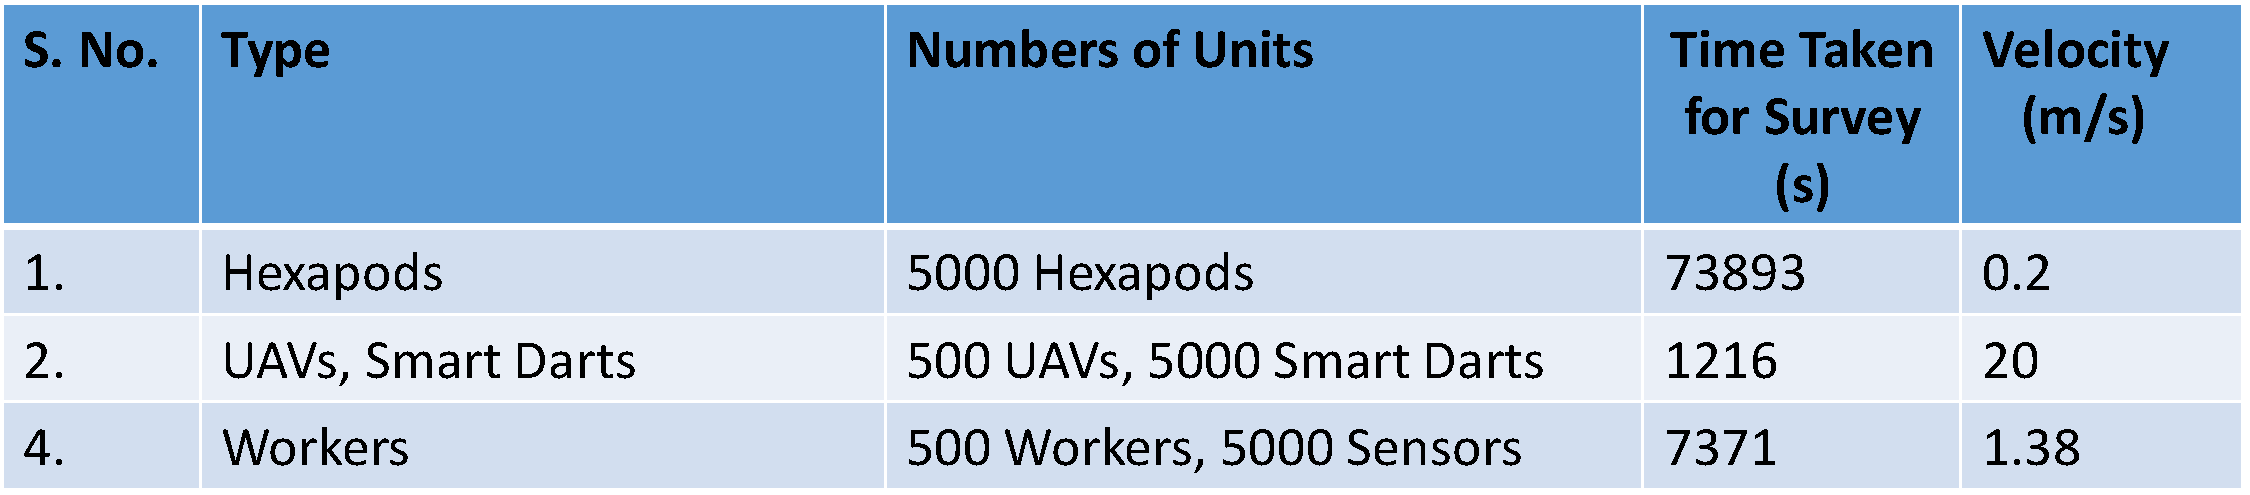
\includegraphics[width=\columnwidth]{simulation_table.pdf}}
 \caption{Comparison of different  deployment modes highlights the efficiency of UAV deployment.} 
 \label{tab:Sim_table}
\end{table}

\begin{figure} \centering
  {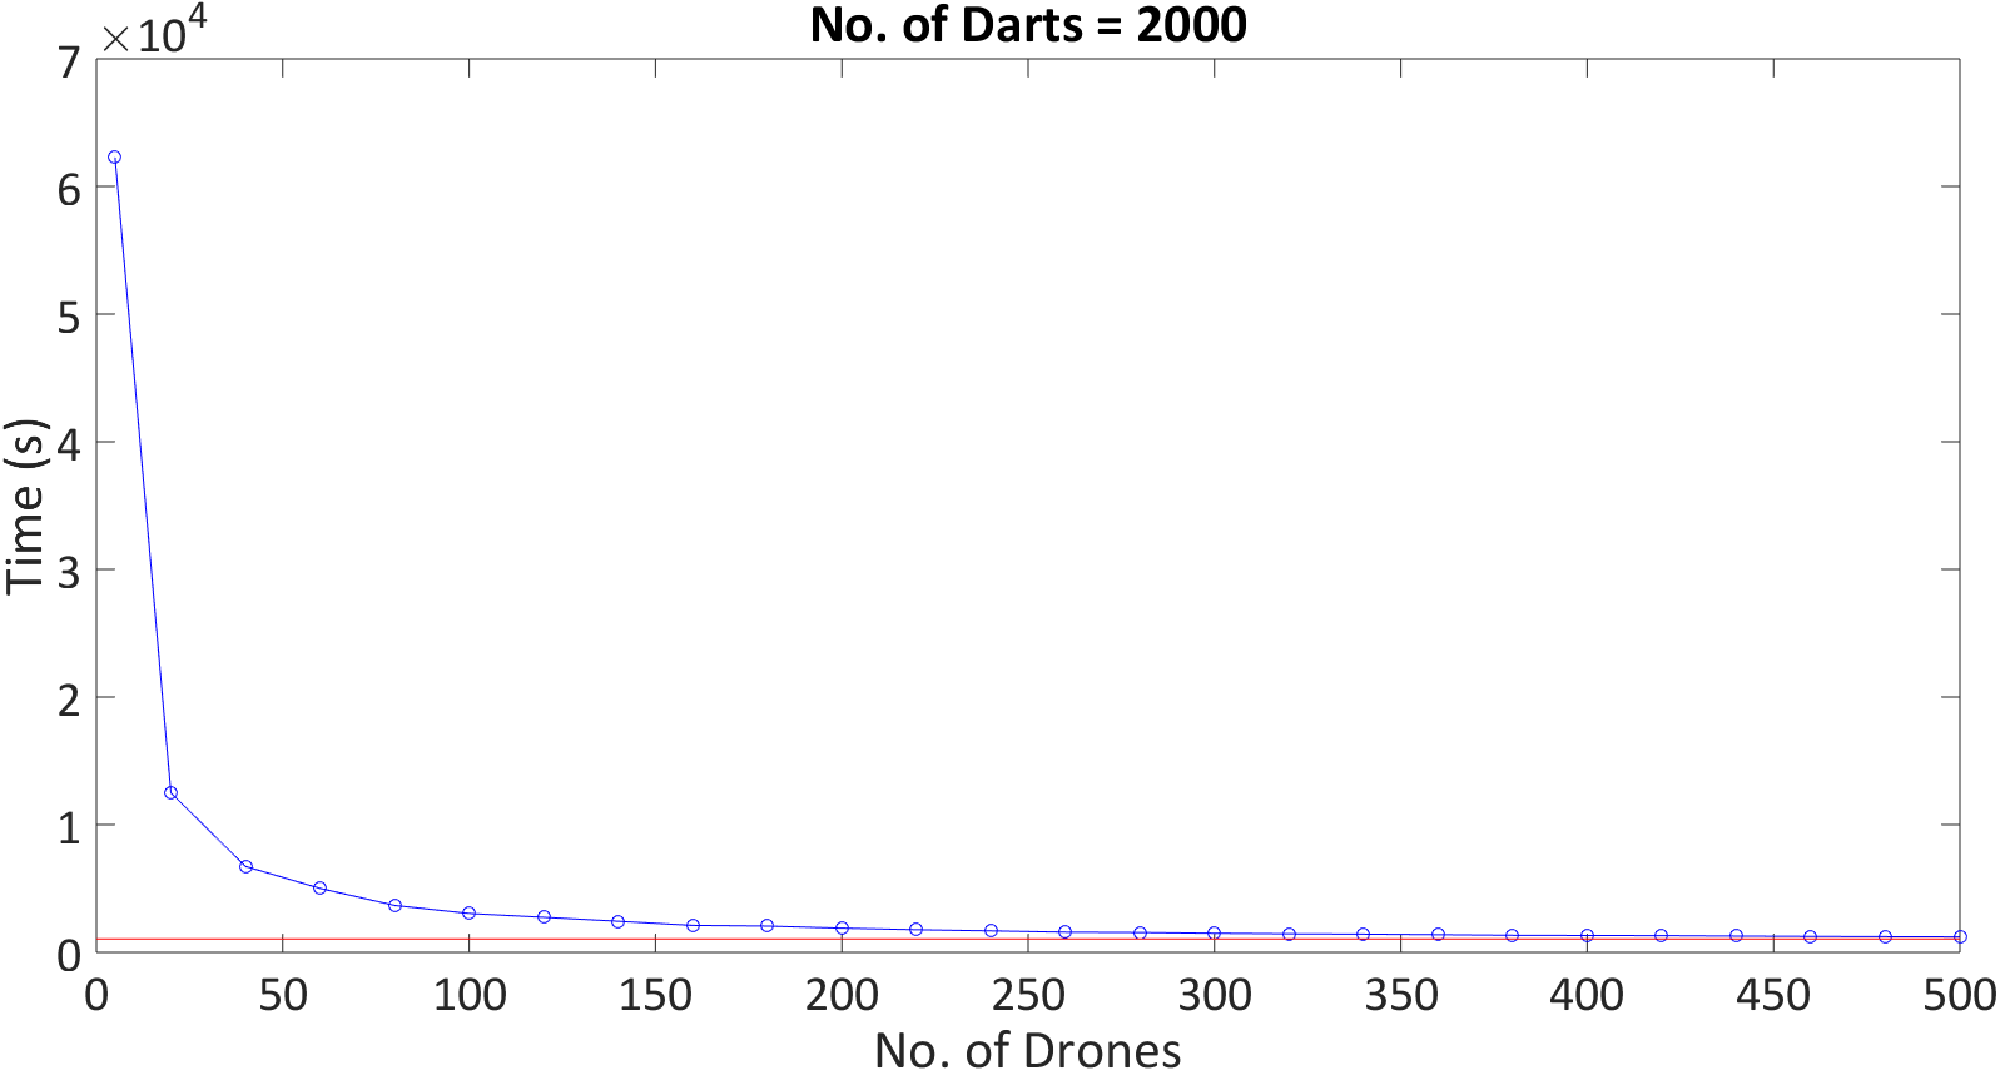
\includegraphics[width=\columnwidth]{DronevsTime.pdf}}
 \caption{Survey time for a 1km x 10 km region for different numbers of UAVs.} 
 \label{fig:DronevsTime}
\end{figure}

\begin{figure} \centering
  {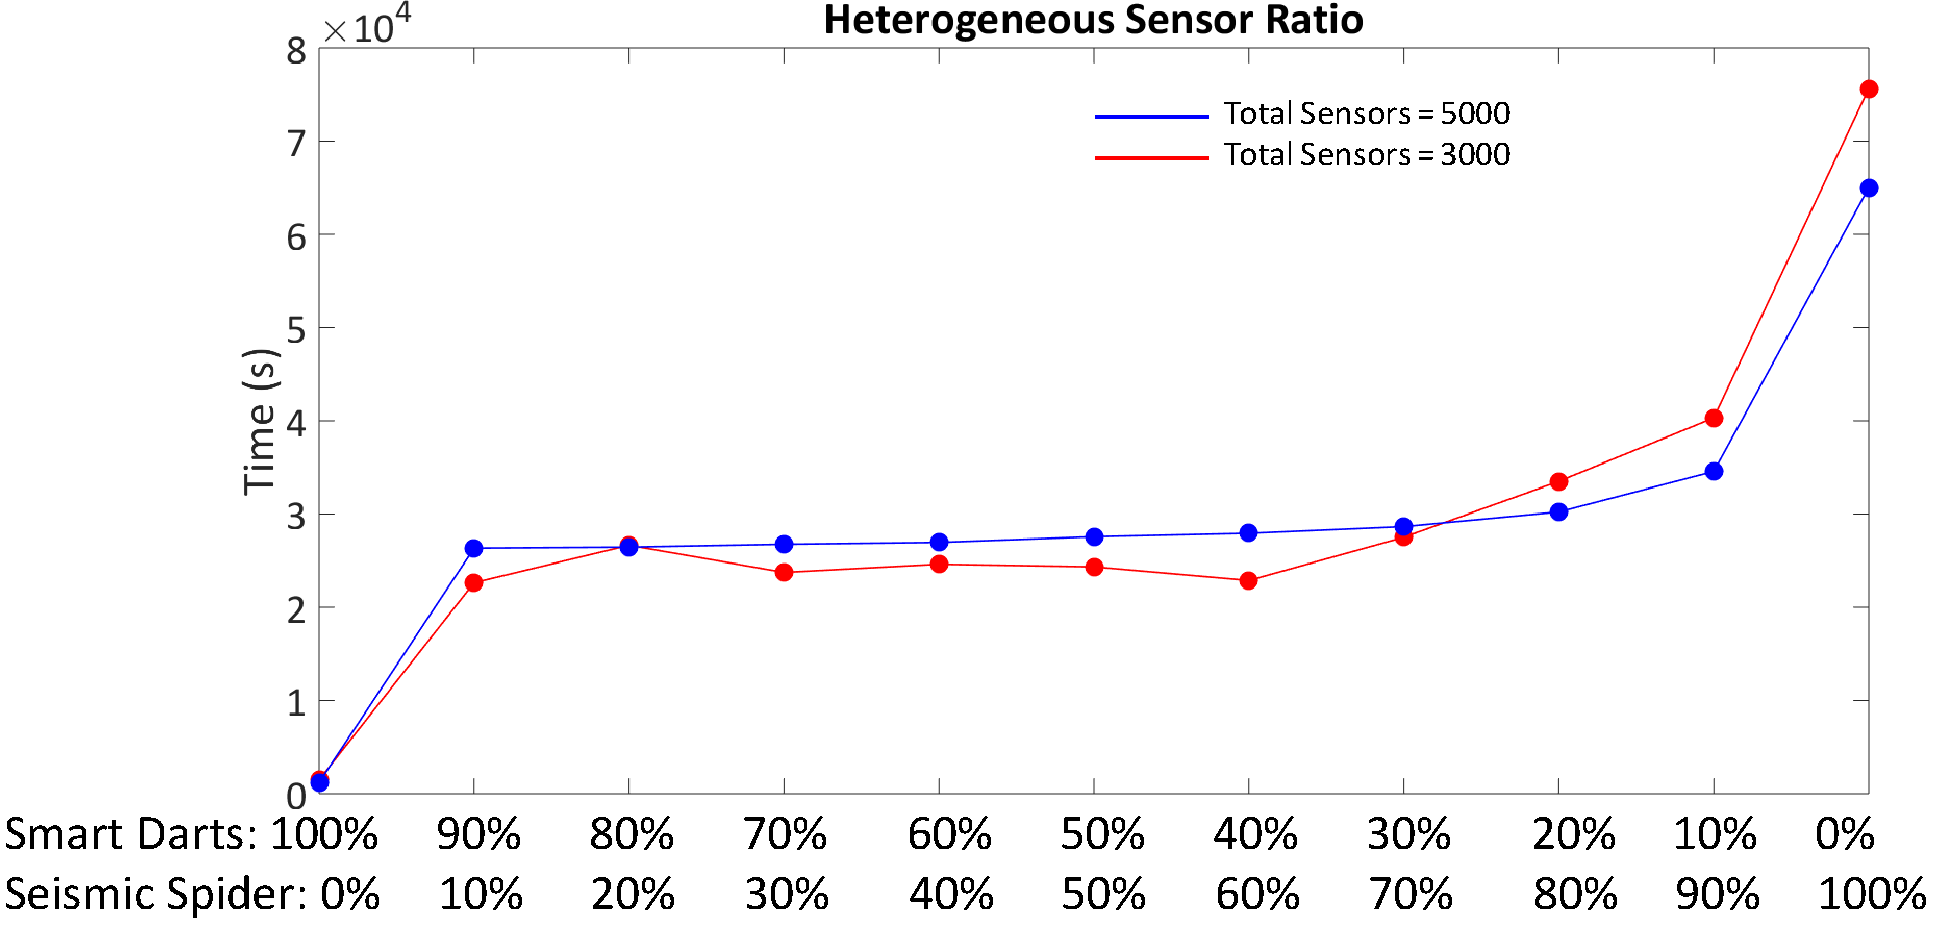
\includegraphics[width=\columnwidth]{het_sen_ratio.pdf}}
 \caption{Survey time for different sensor ratios. The total number of sensors \{5000, 3000\} were kept constant. Ten darts were provided for each UAV. } 
 \label{fig:het_sen_ratio}
\end{figure}

\subsection{Simulation Studies}


A scheduling system to compare  time and costs for seismic surveys with varying numbers of UAVs, SeismicSpiders, SeismicDarts, and human laborers was coded in  {\sc Matlab}, available at \cite{Srikanth2016seismicScheduler}. Frames from four different cases are shown in Fig.~\ref{fig:Sim_overview}.

This tool allows us to examine engineering and logistic trade-offs quickly in simulation.  For example, Fig.~\ref{fig:DronevsTime} assumes a fixed number of darts, and examines the finishing time with $5$ to $500$ UAVs.  The time required decays asymptotically, but $140$ UAVs requires only twice the amount of time required for $500$ UAVs, indicating that $140$ UAVs are sufficient for the task.    
 Substantial cost savings can be obtained by selecting the number of UAVs required to complete within a certain percentage greater than the optimal time.

The tool is useful for comparing the effectiveness of heterogeneous teams.  Table~\ref{tab:Sim_table} compares surveying a $1$ km x $10$ km strip of land with teams of (a) $5000$ SeismicSpiders, (b) $500$ UAVs and $5000$ SeismicDarts, (c) $500$ humans and $5000$ geophones.  Team (b) completed $6$ times faster than team (c). 
  Since SeismicSpiders are  slower than UAVs and humans, and are expensive compared to the SeismicDarts, their use is limited to special occasions. The Seismic UAV has the ability to deploy the SeismicSpider at a given waypoint. This attribute was not considered in the simulation but would improve deployment speed of SeismicSpiders.
   
In Fig.~\ref{fig:het_sen_ratio}, the total number of mobile agents are constant, but the percentage of UAVs and SeismicSpiders are varied. The goal is to analyze ratios of different sensors to optimize cost and time. 10 SeismicDarts were provided for each UAV. Increasing the percentage of UAVs lowers the deployment time. This is obvious since UAVs move at 20 m/s whereas SeismicSpiders move at 0.2 m/s. The difference in velocities makes UAV deployment time efficient. The SeismicSpiders are ideal for hard surface sensing or regions difficult for UAVs to access such as  forests.

